\section{Renormalization group flows}\label{ss:RGflow}

In this section, we turn our attention to the dynamical aspects of entanglement entropy under an RG flow.
We first overview the idea of RG flows as a course graining of microscopic degrees of freedom and detail the motivation and implication of the so-called $\CC$-theorem realizing our intuition that the effective degrees of freedom monotonically decrease along RG flows in the theory space of QFT.
The current status of the $\CC$-theorems in various dimensions will be recapitulated for the readers' convenience.
We then proceed to the proofs for the entropic version of the $c$-theorem in two dimensions and the $F$-theorem in three dimensions.
The monotonicities of $\CC$-functions built from entanglement entropy will be shown as a consequence of the strong subadditivity and Lorentz invariance of QFT.
As a specific example, we consider a free massive scalar field and examine the $F$-theorem by introducing a systematic method of the large mass expansion.
After sketching the attempts to formulate the $\CC$-theorems in higher dimensions, we move onto the holographic descriptions of entanglement under RG flows and reveal the role of entanglement entropy as an order parameter of phase transitions.
We also make a small test of the $F$-theorem in holographic models of RG flows and conclude the section with comments on some exact results for entanglement in supersymmetric field theories.


\subsection{Ordering theories along RG flows}\label{ss:OrderingRG}
In the Wilsonian picture of QFT, the renormalization group transformation takes one theory  to another effective theory by coarse graining the microscopic degrees of freedom heavier than the energy scale of our interest, resulting in a trajectory called an RG flow in the space of QFTs parametrized by coupling constants \cite{Wilson:1973jj,Polchinski:1983gv}.

To be more concrete, let us denote the theory space of QFTs by $\CT$ whose coordinates are given by a set of coupling constants $\{ g_i\}$, and the RG transformation by $\mathfrak{R}_t$ that induces a flow from one theory $T \in\CT$ to another theory $\mathfrak{R}_t\, T$.
The parameter $t \ge 0$ counts how many times the coarse-graining is processed, hence playing a role of time for RG flows.
It will be convenient to relate the RG time $t$ with the energy scale $\mu$ by $t = - \log (\mu/\Lambda)$ where $\Lambda$ is the UV cutoff.
One can follow the trajectory of the RG flow of a given theory $T$ by changing $t$ from the UV ($t=0$) to the IR limit ($\infty$).

The fixed points of RG flows are by definition scale invariant field theories, which are  expected to be CFTs under the assumptions of unitarity and Poincar{\'e} invariance \cite{Nakayama:2013is}.
We thus associate to an RG flow the UV and IR CFTs denoted by $T_\text{UV}$ and $T_\text{IR}$ at $t = 0$ and $t=\infty$ respectively.
There can be multiple RG flows attached to one fixed point depending on the types of perturbation added to the corresponding CFT.
Figure \ref{fig:c-function} illustrates a situation of the theory space with four fixed points $T_1,T_2,T_3$, and $T_4$ represented by the black dots, some of which are connected by RG flows in a nontrivial way.


\begin{figure}[ht]
\centering
		\begin{tikzpicture}[scale=0.7, thick,decoration={
    markings,
    mark=at position 0.5 with {\arrow{>}}}]
		\draw[postaction={decorate}] (0,3)  to [out = -90, in = 165] node[below left] {$\mathfrak R$} (3,0);
		\draw[postaction={decorate}] (0,3)  to [out = 10, in = 115] node[above right] {$\mathfrak R'$} (2,2);
		\draw[postaction={decorate}] (2,2)  to [out = -40, in = 115] node[above right] {$\mathfrak R''$} (3,0);
		\draw[postaction={decorate},dashed] (2,2)  to [out = 40, in = 165] node[above] {$?$}(5,2.5);
		\draw[postaction={decorate},dashed] (5,2.5)  to [out = 250, in = 45] node[below right] {$?$}(3,0);
		\draw[fill=black] (0,3) node[above] {$T_1$} circle (0.1);
		\draw[fill=black] (2,2) node[left] {$T_3$} circle (0.1);
		\draw[fill=black] (5,2.5) node[right] {$T_4$} circle (0.1);
		\draw[fill=black] (3,0) node[below] {$T_2$} circle (0.1);
	\end{tikzpicture}
	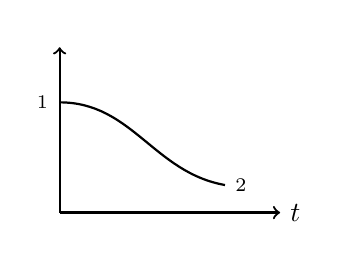
\begin{tikzpicture}[thick,scale=0.7]
		\draw[->] (0,0) -- (4,0) node[right] {$t$};
		\draw[->] (0,0) -- (0,3) node[above] {$\CC$};
		\draw (0,2) node[left] {$\CC_\text{1}$} to [out=0, in=170] (3,0.5) node[right] {$\CC_\text{2}$};
	\end{tikzpicture}
\caption{[Left] An example of RG flows in the theory space $\CT$. The black dots stand for the fixed points of RG flows.
[Right] A $\CC$-function monotonically decreases as the RG time $t$ is increased.
}
\label{fig:c-function}
\end{figure}

Intuitively, physical degrees of freedom must decrease monotonically under any RG flow because massive degrees of freedom are integrated out once the energy scale of the flow becomes below the scale set by the masses.
In other words, we hope to find a function $\CC: \CT \to \BR_{\ge 0}$ that quantifies the effective degrees of freedom of a given theory $T\in \CT$ by a non-negative real number and decreases monotonically along any RG flow on $\CT$:\footnote{The number of degrees of freedom in QFT is conventionally measured by a $\CC$-function in unit of a simplest quantum field such as a free scalar theory.}
\begin{align}\label{c_monotonic_decreasing}
	\frac{\d\, \CC (\mathfrak{R}_t\, T)}{\d t} \le 0 \ .
\end{align}
This type of a function, broadly termed a \emph{$\CC$-function}, brings us a natural interpretation that every RG flow goes downward when its value is regarded as a height on the theory space $\CT$ (Fig.\,\ref{fig:c-function}).
In particular, the UV fixed point is higher than (or at the same altitude as) the IR fixed point:
\begin{align}\label{c_monotonic}
	\CC_\text{UV} \ge \CC_\text{IR} \ ,
\end{align}
where $\CC_i \equiv \CC (T_i)$ are the fixed point values.
As we will see, the fixed point value of a $\CC$-function is often calculable as a scheme-independent quantity in the corresponding CFT without any information around the point.
If this is the case, the inequality \eqref{c_monotonic} constrains the dynamics of RG flows as follows.
Suppose there are two CFTs $T_3$ and $T_4$ in the theory space as in Fig.\,\ref{fig:c-function}, and we are interested in whether there exists an RG flow interpolating them.
In principle, we could perturb one of the theories, e.g., $T_3$, by relevant operators and see if it triggers an RG flow toward the other $T_4$ by perturbative calculations.
On the other hand, if the fixed point values $\CC_3$ and $\CC_4$ are available to us and it turns out that $\CC_3 < \CC_4$, then we can conclude, without any perturbative calculation, that there are no RG flows from $T_3$ to $T_4$ just by resorting to the inequality \eqref{c_monotonic}.

We are thus able to characterize a $\CC$-function by the following conditions:
\begin{itemize}
\item $\CC$ is a function of a renormalization scale $\mu = \Lambda\, e^{-t}$ that we can tune by hand.
\item $\CC$ is well-defined for any QFT, independent of the types of field contents and their interactions.
\item $\CC$ is a monotonic function of the renormalization time $t$ for any unitary and Lorentz invariant QFT in one of the following senses \cite{Barnes:2004jj,Gukov:2015qea}:
	\begin{itemize}
	\item[(i)] [Weak version] The fixed point value of $\CC$ should decrease along RG flows as in Eq.\, \eqref{c_monotonic}.
	\item[(ii)] [Stronger version] $\CC$ monotonically decreases along the entire RG flow as in Eq.\,\eqref{c_monotonic_decreasing}.
	\item[(iii)] [Strongest version] $\CC$ is a potential that generates RG flows:
		\begin{align}
			\beta_i (g) = G_{ij}(g)\,\frac{\partial \CC}{\partial g_j} \ ,
		\end{align}
		where $\beta_i (g) \equiv - \d g_i /\d t$ and $G_{ij}(g)$ is a positive-definite metric on the theory space $\CT$.
	\end{itemize}
\end{itemize}
Here we distinguish the three versions of a $\CC$-function in increasing order of strength for completeness.
The weak version follows from the stronger one by integrating Eq.\,\eqref{c_monotonic_decreasing} along the flow.
The stronger version is implied by the strongest one too,
\begin{align}
	\frac{\d\,\CC}{\d t} = - \beta_i \,\frac{\partial\,\CC}{\partial g_i} = - G_{ij}\,\frac{\partial\,\CC}{\partial g_i} \frac{\partial\,\CC}{\partial g_j}  \le 0 \ .
\end{align}


While the existence of a $\CC$-function may be taken for granted from the physical point of view, the problem is how to construct such a well-behaved function satisfying the aforementioned properties.
Indeed the construction of a $\CC$-function for QFT in dimensions higher than $2$ has been a long-standing problem for three decades since the initiating work by \textcite{Zamolodchikov:1986gt}, and was successfully settled down recently in only three and four dimensions.

One possible approach to this problem is to formulate a set of axioms that guarantee the existence of a $\CC$-function in any dimension without any explicit construction.
The power of an axiomatic approach is well demonstrated in axiomatic thermodynamics whose most important consequence is the very existence of a unique entropy function that never decreases under adiabatic processes and characterizes thermal equilibrium states when represented as a function of extensive variables such as energy and volume [see, e.g., \textcite{Lieb:1997mi} for a review of the subject].
In fact, there are considerable similarities between the theory space of QFT and the state space of thermodynamics.
For instance, the irreversibility of an RG flow between two fixed points $T_a,T_b \in \CT$ corresponds to an irreversible adiabatic process $a \to b$ that takes one equilibrium state $a$ to the other $b$.
A partial list of the analogies between thermodynamics and QFT is shown in Table\,\ref{tab:Analogy}.
It would be of great interest to translate the set of axioms for equilibrium thermodynamics into the language of QFT and examine to what extent the formulation of an entropy function carries over to the construction of a $\CC$-function.
We will not address this possibility any further in this review and leave it to future investigations.
Instead, we will take a constructive approach for a $\CC$-function in the subsequent sections.

\begin{table}
\caption{\label{tab:Analogy}An analogy between thermodynamics and QFT.}
\begin{ruledtabular}
\begin{tabular}{cc}
	Thermodynamics & QFT \\
	\hline
	Equilibrium states  & Conformal fixed points\\
	$a,b$ & $T_a, T_b$ \\
	Union of two states & Coupling of two theories\\
	$a+b$ & $T_a$ and $T_b$ \\
	Irreversible adiabatic process & RG flow \\
		$a\rightarrow b$ & from $T_a$ to $T_b$\\
	Entropy function & $\CC$-function
\end{tabular}
\end{ruledtabular}
\end{table}


\subsection{List of $\CC$-theorems}
We now provide a list of the known $\CC$-theorems and related conjectures in various dimensions along with comments on their historical backgrounds.

\subsubsection{Two dimensions}
\textcite{Zamolodchikov:1986gt} proved his celebrated $c$-theorem in the following form.

\begin{theorem*}[Zamolodchikov's $c$-theorem]
In two-dimensional renormalizable QFTs, there exists Zamolodchikov's $c$-function $c(g_i, \mu)$ that depends on a set of dimensionless coupling constants $\{ g_i\}$ and the energy scale $\mu (= \Lambda\,e^{-t})$, satisfying the following properties:
\begin{enumerate}
\item It takes the same value as the central charge $c$ of the CFT corresponding to each fixed point of RG flows:
	\begin{align}
		c(g_i, \mu)|_\mathrm{CFT} = c \ .
	\end{align}
\item It monotonically decreases along any RG flow:
	\begin{align}
		\frac{\d\, c(g_i, \mu)}{\d t} = - \mu \frac{\d\, c(g_i, \mu)}{\d\mu} \le 0 \ .
	\end{align}
\item It is stationary only at the fixed points:
	\begin{align}
		\frac{\partial\, c(g_i, \mu)}{\partial g_i}\bigg|_\mathrm{CFT} = 0 \ .
	\end{align}
\end{enumerate}
\end{theorem*}
Hence, Zamolodchikov's $c$-theorem falls into the strongest version in the terminology introduced in the previous section \cite{Friedan:2009ik}.
The Zamolodchikov's $c$-function can be built explicitly from the two-point correlation functions of the stress-energy tensor in two dimensions, and the monotonicity follows from the reflection positivity of the correlator.


\subsubsection{Three dimensions}

Given the fact that Zamolodchikov's $c$-function gives the central charge at the fixed points, it is tempting to look for counterparts of the two-dimensional central charge in $d>2$ dimensions.
Let us consider a few candidates for central charges that can be defined irrespective of dimensionality.
\begin{enumerate}
\item[$(a)$]
A ``thermal central charge" $C_\text{Therm}$ as a coefficient of the thermal free energy density $f_\text{Therm}$ at finite temperature $T$ defined by
\begin{align}\label{Thermal_C}
	f_\text{Therm} \sim C_\text{Therm}\, T^d  \ .
\end{align}
\item[$(b)$]
The coefficient $C_T$ for the two-point function of the stress-energy tensor in Eq.\,\eqref{TTCor}.
\item[$(c)$]
The central charges $A$, $B_i$ for the conformal anomalies defined by Eq.\,\eqref{WeylAnomaly} that exist only in even $d$ dimensions.
\end{enumerate}
In $d=2$ dimensions, all of these are known to be proportional to the central charge $C_\text{Therm} \propto C_T \propto A \propto c$ for CFT, but they do not generally have linear relations in higher dimensions.

The possibility $(a)$ of adopting the thermal central charge $C_\text{Therm}$ as a measure of degrees of freedom was studied by \textcite{Sachdev:1993pr} for the three-dimensional $\O(N)$ vector model in the large-$N$ limit.
This model has the RG flow from the Gaussian fixed point $T_\text{Gaussian}$, where all the $N$ scalar fields are free and massless, to the critical $\O(N)$ (interacting) fixed point $T_\text{critical}$ by keeping the renormalized masses vanishing.
Perturbing the critical $\O(N)$ fixed point by giving the scalars negative mass squared terms triggers the RG flow to the $\O(N-1)$ symmetric (Goldstone) fixed point $T_\text{Goldstone}$ with $N-1$ massless free scalar fields (Goldstone modes).\footnote{There is one massive scalar field that decouples at the Goldstone fixed point.}
If the thermal central charge measures the degrees of freedom correctly, we expect them to be ordered along the RG flow $C_\text{Therm} (T_\text{Gaussian}) > C_\text{Therm} (T_\text{critical}) > C_\text{Therm} (T_\text{Goldstone})$.
The thermal central charges at the Gaussian and Goldstone fixed points are simply given by $C_\text{Therm} (T_\text{Gaussian}) = N\,C_\text{Therm}(T_\text{scalar})$ and $C_\text{Therm} (T_\text{Goldstone}) = (N -1)\,C_\text{Therm}(T_\text{scalar})$ as consistent with the RG flow, where  $T_\text{scalar}$ is a real massless free scalar field theory.
On the other hand, the large-$N$ analysis showed $C_\text{Therm} (T_\text{critical}) = \left(4N/5 + O(1)\right)\,C_\text{Therm}(T_\text{scalar})$, which can be less than the IR value $C_\text{Therm} (T_\text{Goldstone})$ for large $N$ and ruled out the possibility of $C_\text{Therm}$ being the fixed point value of a $\CC$-function \cite{Sachdev:1993pr}.

The option $(b)$ employing the coefficient $C_T$ as a fixed point value of a $\CC$-function was suggested by \textcite{Petkou:1995vu} based on the result $C_T (T_\text{critical}) = \left( N - 40/(9\pi^2) \right)\, C_T (T_\text{scalar})$ consistent with the RG flows described for the $\O(N)$ vector model.
This possibility was explored by \textcite{Nishioka:2013gza} more systematically for $\CN =2$ supersymmetric field theories in three dimensions that allows the exact calculation of $C_T$ due to the supersymmetric localization technique.
In that work it was shown that a supersymmetric analog of the $\O(N)$ vector model ($\CN=2$ Wess-Zumino model) can be a counterexample for the ``$C_T$"-theorem.
Another counterexample was also found by \textcite{Fei:2014yja} by examining the RG flows in the five-dimensional $\O(N)$ symmetric scalar field theory with the $\O(N)$ symmetric interacting fixed point.


In three dimensions, there exists no conformal anomaly; hence the third option $(c)$ is unavailable on its own.
Alternatively, a proposal was made by \textcite{Jafferis:2011zi} [and independently by \textcite{Myers:2010xs,Myers:2010tj} in a different form from the holographic viewpoint] based on the extremization principle of the supersymmetric partition function \cite{Jafferis:2010un}, which is now known as the $F$-theorem,
\begin{theorem*}[$F$-theorem]
In three-dimensional QFTs, there exists a function $\CF(g_i, \mu)$ on the theory space satisfying the following properties:
\begin{enumerate}
\item It takes the same value as the sphere free energy $F$ of the CFT corresponding to each fixed point of RG flows,
	\begin{align}\label{REE_F}
		\CF(g_i, \mu) |_\mathrm{CFT} = F \ ,
	\end{align}
	where $F=-\log |Z[\BS^3]|$ and $Z[\BS^3]$ is the (renormalized) Euclidean partition function on $\BS^3$.
\item It is a monotonically decreasing function under any RG flow,
	\begin{align}\label{REEMonotonicity}
		\frac{d\,\CF}{d\,t}  = - \mu \frac{\d\,\CF}{\d\mu} \le 0 \ .
	\end{align}
\end{enumerate}
\end{theorem*}
This statement can be regarded as a variant of the third option $(c)$ since we can extract the type $A$ central charge of the conformal anomaly from the sphere partition function $A \propto \log Z[\BS^d]$ in even dimensions.


While the $F$-theorem was originally stated in the weak form $F_\mathrm{UV} \ge F_\mathrm{IR}$, a perturbative argument \cite{Klebanov:2011gs,Yonekura:2012kb} suggests the sphere free energy is the strongest version of a $\CC$-function.
Strong evidence supporting the $F$-theorem was given for $\CN=2$ supersymmetric theories with $\U(1)_R$ symmetry, where
the sphere free energy $F$ is shown to be locally maximized at RG fixed points \cite{Jafferis:2010un,Closset:2012vg} unless there is no accidental symmetry at the IR fixed point [see also the review by \textcite{Pufu:2016zxm} for details].
A nonperturbative proof of the strong version of the $F$-theorem was given by \textcite{Casini:2012ei} by exploiting the unexpected relation between the free energy and  the entanglement entropy of a disk we derived in Eq.\,\eqref{EE_F}. 
We outline the proof and the implications in Sec. \ref{ss:Ftheorem}.


\subsubsection{Four dimensions}
Seeking for a $\CC$-theorem in four dimensions has a long history starting from the conjecture [of the type $(c)$ in Sec. \ref{ss:OrderingRG}] by \textcite{Cardy:1988cwa} for the $a$-theorem.
\begin{theorem*}[$a$-theorem]
In four-dimensional QFTs, the type $A$ central charge $a$ of the conformal anomaly decreases along any RG flow
\begin{align}\label{a_theorem_claim}
a_\mathrm{UV} \ge a_\mathrm{IR} \ .
\end{align}
\end{theorem*}
This weak version of the $a$-theorem has passed a number of tests over the years in perturbative QFTs \cite{Osborn:1989td,Jack:1990eb} and was given an evidence for $\CN=1$ supersymmetric theories by the $a$-maximization method that implies the strongest $a$-theorem \cite{Intriligator:2003jj,Barnes:2004jj}.
A proof of the $a$-theorem without relying on supersymmetry was presented more recently by \textcite{Komargodski:2011vj} who connect the difference of the $a$-coefficient with the scattering amplitude of four dilaton fields that naturally couple to the stress-energy tensor [see also \cite{Komargodski:2011xv}].
Interestingly the unitarity of the scattering amplitude turns out to guarantee the inequality \eqref{a_theorem_claim} in their proof.

Recently, an alternative proof of the $a$-theorem was given by \textcite{Casini:2017vbe} who resort to the monotonicity of entanglement as in the case of the $F$-theorem.
We touch on the proof in Sec. \ref{ss:C_theorem_Higher}.

Finally, a few comments on the other possibilities are in order:
\begin{enumerate}
\item[$(a)$] The thermal central charge $C_\text{Therm}$ does not satisfy a $\CC$-theorem in a class of four-dimensional gauge theories that are not asymptotically free at UV \cite{Appelquist:1999hr}.
\item[$(b,c)$] The $C_T$ coefficient of the stress-tensor two-point function is proportional to the type $B$ central charge $c$, $C_T \propto c$, in four dimensions \cite{Osborn:1993cr}.
The latter was extensively studied in supersymmetric and nonsupersymmetric theories and many counterexamples are known in a typical class of gauge theories  \cite{Cappelli:1990yc,Anselmi:1997am}.
\end{enumerate}


\subsubsection{Higher dimensions}
Given the success in $d\le 4$ dimensions, one may be tempted to extend a $\CC$-theorem to higher dimensions $d>4$.
This problem was less explored than the lower-dimensional cases, but once formulated it will provide us a unifying picture of RG flows in QFT irrespective of dimensionality.
It is too early to survey the whole subject as it is still under active investigation.
We thus comment only on the two following promising conjectures\footnote{See also \textcite{Gukov:2015qea,Gukov:2016tnp} for a recent discussion on  constraining RG flows by topological data of the theory space.
}:
\begin{itemize}
\item The $a$-theorem in higher even dimensions postulates the monotonicity of the type $A$ central charge for the conformal anomaly under RG flows.
There is supporting evidence for the $a$-theorem from holography \cite{Myers:2010xs,Myers:2010tj} and even proofs for a certain class of supersymmetric field theories in six dimensions \cite{Cordova:2015fha,Cordova:2015vwa}.
\item The $F$-theorem in higher odd dimensions was suggested by \textcite{Klebanov:2011gs,Myers:2010xs,Myers:2010tj} and further incorporated into the generalized $F$-theorem proposal \cite{Giombi:2014xxa} that interpolates between the $F$-theorem and the $a$-theorem in noninteger dimensions.
A few examples supporting the $F$-theorem in five dimensions are presented by \textcite{Jafferis:2012iv,Fei:2014yja}.
\end{itemize}


\subsection{The entropic $c$-theorem in $(1+1)$ dimensions}

We shall prove the strong version of the $\CC$-theorem in two dimensions
by constructing a $\CC$-function built from entanglement entropy.
A $\CC$-function should be well-defined for any QFT and monotonically decreases as  the energy scale $\mu$ is lowered while fixing the size of a system (e.g., an entangling region).
One good candidate for it is the entanglement entropy $S(R)$ of an interval of width $R$ in $(1+1)$ dimensions (see Fig.\,\ref{fig:2dCFT_EE2}).
\begin{figure}[h]
\centering
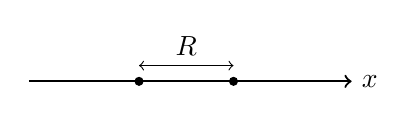
\begin{tikzpicture}
\filldraw [fill=black] (-0.6,-1.8) circle (0.05) ;
\filldraw [fill=black] (0.6,-1.8) circle (0.05);
\draw[<->] (-0.6,-1.6)  -- node[above] {$R$}(0.6,-1.6);
\draw[thick, ->] (-2, -1.8) -- (2.1, -1.8) node[right] {$x$};
\end{tikzpicture}
\caption{An interval of width $R$ as an entangling region.}
\label{fig:2dCFT_EE2}
\end{figure}

Instead of tuning the energy scale $\mu$ with the system size fixed, 
we would rather change the size $R$ to trigger an RG flow while fixing $\mu$.
In this picture, we can probe the physics at the UV and IR scales by small and large intervals respectively.
The conditions for a function $c_E(R)$ being a $\CC$-function are restated in the following form:
\begin{enumerate}
\item $c_E(R)$ coincides with the central charge $c$ of CFT$_2$ at a fixed point of an RG flow,
	\begin{align}
		c_E(R) |_\text{CFT} = c \ .
	\end{align}
\item $c_E(R)$ is a monotonically decreasing function under any RG flow,
	\begin{align}\label{EntropicMonotonicity}
		c_E'(R)\le 0 \ .
	\end{align}
\end{enumerate}
Recalling from Eq.\,\eqref{EE_CFT2}, the entanglement entropy of the interval in CFT$_2$ becomes\footnote{We can redefine the UV cutoff $\epsilon$ so as to remove a finite term in Eq.\,\eqref{EE_CFT2}.}
\begin{align}
S(R)|_\text{CFT} = \frac{c}{3}\log \frac{R}{\epsilon} \ ,
\end{align}
where the central charge $c$ appears as a coefficient of the logarithmic divergence.
It follows that we can introduce the \emph{entropic $c$-function} \cite{Casini:2004bw} satisfying the first condition,
\begin{align}\label{Entropic_C}
c_E(R) \equiv 3R\, S'(R) \ .
\end{align}
Note that the entropic $c$-function is well-defined for \emph{any} QFT as it is built from the entanglement entropy of an interval.
It should also be stressed that the entropic $c$-function is free from the UV divergence as there is only logarithmic divergence in two dimensions, and it always takes a finite value in contrast to the entanglement entropy itself.

In order to prove that the monotonicity of the entropic $c$-function, Eq.\,\eqref{EntropicMonotonicity}, we consider two intervals $A$ and $C$ on the light rays $t=\pm x$ (the dashed lines) and an interval $B$ of width $r$ on a time slice $t=0$ as in Fig.\,\ref{fig:EntropicC}.
More precisely we choose the three regions as follows:
\begin{align}
	\begin{aligned}
		A &= \left\{ t = -x, \, -\frac{R}{2} \le x \le - \frac{r}{2} \right\} \ , \\
		B&= \left\{ t = 0, \, - \frac{r}{2} \le x \le \frac{r}{2} \right\} \ , \\
		C&= \left\{ t = x, \,  \frac{r}{2} \le x \le \frac{R}{2} \right\} \ .
	\end{aligned}
\end{align}
%
\begin{figure}[htbp]
\centering
	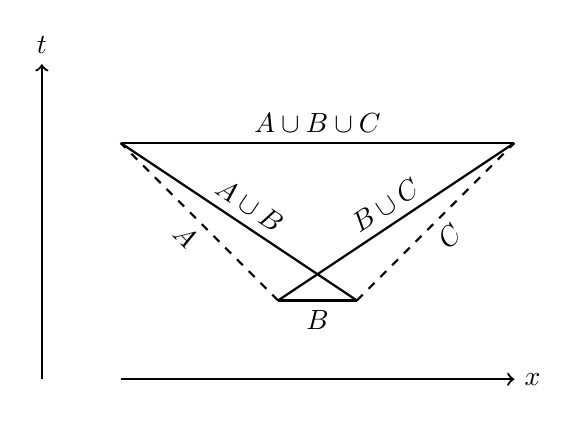
\begin{tikzpicture}[thick]
		\draw[->] (0,0) --++ (5,0) node[right] {$x$};
		\draw[->] (-1,0) --++ (0,4) node[above] {$t$};
		\draw (2,1)-- node[below] {$B$} ++(1,0);
		\draw (0,3)-- node[above] {$A\cup B \cup C$} ++(5,0);
		\draw[dashed] (2,1) -- node[below, sloped] {$A$}++(-2,2);
		\draw[dashed] (3,1) -- node[below, sloped] {$C$} ++(2,2);
		\draw (2,1) -- node[above,sloped] {$B\cup C$} (5,3);
		\draw (3,1) -- node[above,sloped] {$A\cup B$} (0,3);
	\end{tikzpicture}
\caption{A proof of the entropic $c$-theorem. Two intervals $A$ and $C$ are on the light rays $t=\pm x$ while an interval $B$ is on a time slice $t=0$.}
\label{fig:EntropicC}
\end{figure} 
Entanglement entropy is invariant under unitary time evolution and hence is Lorentz invariant in QFT.
We thus are able to use the boosted interval connecting the left end point of $A$ and the right end point of $B$ to calculate the entanglement entropy of the union $A\cup B$.
Similarly the entanglement entropy of the union $B\cup C$ is equal to that of the boosted interval connecting the left end point of $B$ and the right end point of $C$,\footnote{The diffeomorphism invariant length $\Delta R$ between two points $(t,x)$ and $(t+\Delta t, x+\Delta x)$ is defined by
\begin{align}
	\D R= \sqrt{- (\D t)^2 + (\D x)^2} \ .
\end{align}
}
\begin{align}
	S_{A\cup B} = S_{B\cup C} = S\left(\sqrt{rR}\right) \ .
\end{align}
The union of the three regions $A\cup B\cup C$ can also be time-evolved into the interval of width $R$ at $t=(R-r)/2$.
Hence the entanglement entropies of $A\cup B\cup C$ and $B$ are
\begin{align}
	S_{A\cup B\cup C} = S(R) \ , \qquad S_B = S(r) \ .
\end{align}

Now we apply the strong subadditivity Eq.\,\eqref{SSA} and find the inequality,
\begin{align}\label{ECSSA}
 S(R) + S(r) \le 2 S\left(\sqrt{rR}\right)\ .
\end{align}
We can reduce it in the limit $r\to R$ to \cite{Casini:2004bw}\footnote{See also \textcite{Bhattacharya:2014vja} for the generalization of this argument to prove the positivity of the entanglement density.}
\begin{align}\label{ECmonotonic}
\frac{c_E'(R)}{3} = S'(R) + RS''(R) \le 0 \ ,
\end{align}
which is actually what we wanted to prove, Eq.\,\eqref{EntropicMonotonicity}.
It is worthwhile to emphasize that conformal symmetry plays no roles in the proof of the inequality \eqref{ECmonotonic}, and hence it is valid for \emph{any} QFT as it follows from the strong subadditivity of entanglement entropy and Lorentz invariance in QFT.


We note that the entropic $c$-function Eq.\,\eqref{Entropic_C} is not stationary at the UV fixed point for a free massive scalar theory \cite{Casini:2005zv}; hence it is an example of the stronger $\CC$-theorem in the terminology of Sec. \ref{ss:OrderingRG}.
It behaves quite differently from Zamolodchikov $c$-function under RG flows although they coincide at conformal fixed points.
It remains open whether there exists a strongest $\CC$-function built from entanglement entropy.


\subsection{The $F$-theorem in $(2+1)$ dimensions}\label{ss:Ftheorem}
We adapt the argument for the entropic $c$-theorem to the proof of the strong version of the $F$-theorem in a $(2+1)$-dimensional QFT.
A counterpart of the entropic $c$-function will be introduced as the renormalized entanglement entropy $\CF$ \cite{Liu:2012eea}.
We content ourselves with outlining the proof of the monotonicity of $\CF$ and leave the technical details to the original paper \cite{Casini:2012ei}.
After examining the UV and IR behaviors of $\CF$, we discuss the possibility of the strongest version of the $F$-theorem.


\subsubsection{A sketch of the proof}
The nonperturbative proof of the $F$-theorem goes in parallel with that of the entropic $c$-theorem in the previous section.
To this end, we construct a function $\CF(R)$ from the entanglement entropy of a disk satisfying the following:
\begin{enumerate}
\item $\CF(R)$ coincides with the sphere free energy $F$ of CFT$_3$ at a fixed point of an RG flow,
	\begin{align}\label{REE_F_proof}
		\CF(R) |_\text{CFT} = F \ .
	\end{align}
\item $\CF(R)$ is a monotonically decreasing function under any RG flow,
	\begin{align}\label{REEMonotonicity_proof}
		\CF'(R)\le 0 \ .
	\end{align}
\end{enumerate}
The key in finding such a function is the relation \eqref{EE_F} between the sphere free energy $F$ and the entanglement entropy $S(R)$ of a disk of radius $R$ for CFT$_3$,
\begin{align}\label{S_F}
S(R)|_\text{CFT} = \alpha \frac{2\pi R}{\epsilon} - F \ ,
\end{align}
where $\alpha$ is a theory-dependent constant.
In three dimensions, the UV divergence of entanglement entropy $S(R)$ is of order $O(1/\epsilon)$ for any QFT, and it is always proportional to the radius $R$ of the disk due to the area law.
We want to regularize the divergence as in the entropic $c$-function Eq.\,\eqref{Entropic_C}, thus
introducing the \emph{renormalized entanglement entropy} or the $\CF$-function  \cite{Liu:2012eea}
\begin{align}\label{REE}
\CF (R) \equiv (R\, \partial_R - 1) S(R) \ .
\end{align}
Then we see the first condition Eq.\,\eqref{REE_F_proof} for $\CF$ being a $\CC$-function immediately follows from Eq.\,\eqref{S_F}.


Furthermore, \textcite{Casini:2012ei} completed a proof of the $F$-theorem by showing the monotonicity of $\CF$, Eq.\,\eqref{REEMonotonicity_proof}, with the strong subadditivity for any Lorentz invariant field theory.
We only sketch the proof of the inequality Eq.\,\eqref{REEMonotonicity_proof}, leaving the technical details to the original paper \cite{Casini:2012ei} [see also \textcite{Casini:2015woa} for a proof using the mutual information].

The point for proving the entropic $c$-theorem was the choice of the boosted intervals whose union and intersection are intervals of different widths at different time slices as in Fig.\,\ref{fig:EntropicC}.
In order to extend the previous argument to the present case, we have to choose a set of boosted disks touching on the null cone, whose union and intersection approximate disks of different radii, say, $R$ and $r\, (\le R)$ (see Fig.\,\ref{fig:Fproof}).
Clearly an infinite number of boosted disks are needed to realize such a situation.
Hence, we begin with $N$ boosted disks labeled by $X_i~(i=1,\cdots, N)$ whose diffeomorphism invariant radii are $\sqrt{r R}$ and apply to them the inequality obtained by the repeated use of the strong subadditivity 
\begin{align}\label{SSA_general}
\begin{aligned}
	S_{\cup_i X_i} &+ S_{\cup_{\{i,j\}} X_{ij}} \\
		& + S_{\cup_{\{i,j,k\}} X_{ijk}} + \cdots + S_{\cap_i X_i} \le \sum_i S_{X_i} \ ,
\end{aligned}
\end{align}
where we used the shorthand notation $X_{ij\cdots k} \equiv X_i \cap X_j \cap \cdots \cap X_k$.
There are $N$ terms on the left-hand side, each of which gives a disk entropy of a radius ranging from $r$ to $R$.
Dividing by $N$ on both sides, the sum on the left-hand side approaches an integral in the $N\to \infty$ limit,
\begin{align}
	\frac{1}{\pi} \int_0^\pi \d\theta \, S\left(\frac{2rR}{R + r - (R-r)\cos\theta} \right) \le S\left( \sqrt{rR} \right) \ .
\end{align}
Letting $R = r - \epsilon$ and expanding both  sides at $\epsilon = 0$, one finds $S''(R)\le 0$ at order $O(\epsilon^2)$,
\begin{align}\label{REEmonotonic}
\CF'(R) = R\,S''(R) \le 0 \ ,
\end{align}
which is the other necessary condition Eq.\,\eqref{REEMonotonicity_proof} for $\CF$ being a $c$-function in three dimensions.
We again stress, as in the case of the entropic $c$-theorem in two-dimensions, that the inequality \eqref{REEmonotonic} is valid for \emph{any} QFT as the proof does not rely on conformal symmetry at all.

\begin{figure}[htbp]
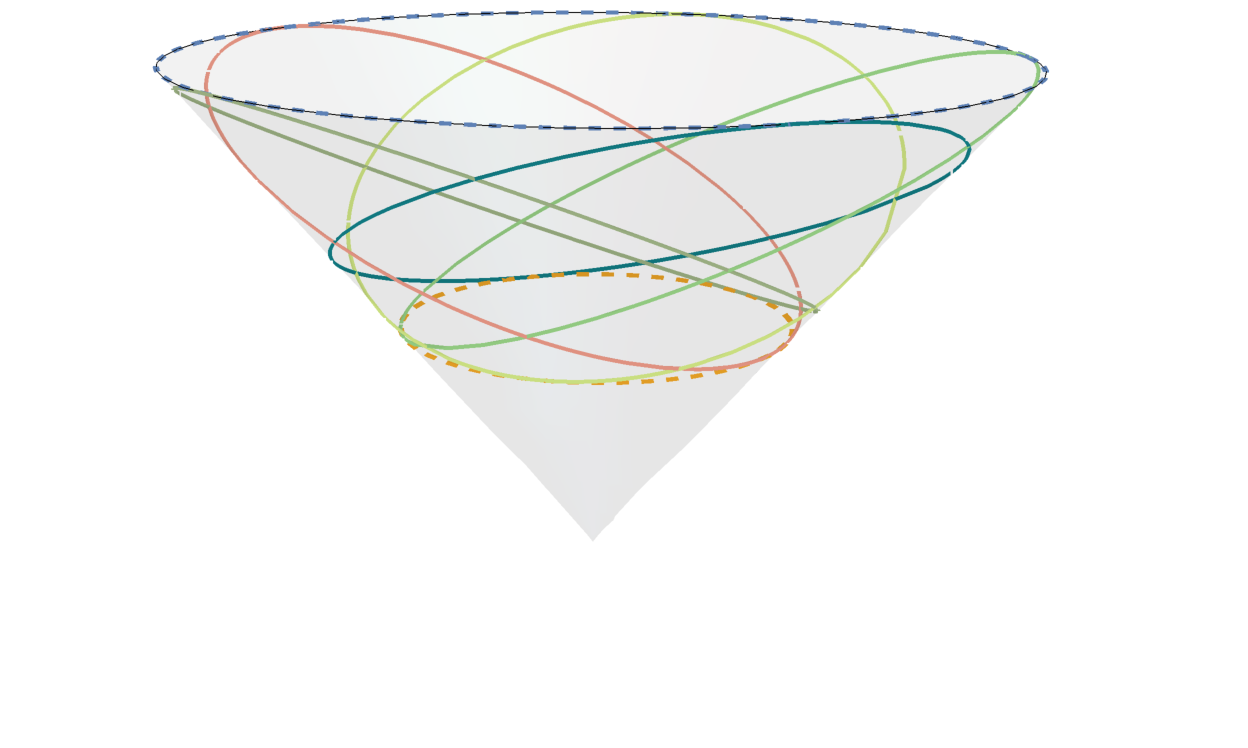
\includegraphics[width=7cm]{Fproof.pdf}
\caption{\label{fig:Fproof} $N=5$ boosted disks of radii $\sqrt{rR}$ touching on the null cone in gray color.
The dashed curves are circles of radii $R$ and $r$ at constant time slices $t=R$ and $r$, respectively.
}
\end{figure}


\subsubsection{Constraints from the $F$-theorem}

As applications of the $F$-theorem, we want to constrain the phase diagram of 
noncompact QED$_3$ coupled to $2N_f$ two-component Dirac fermions of unit charges $\psi^i~(i=1,\cdots, 2N_f)$ \cite{Grover:2012sp,Giombi:2015haa}.
This theory enjoys the $\SU(2N_f)$ global symmetry and flows to the conformal phase for large $N_f$ at the IR fixed point.
On the other hand, the theory is suspected to exhibit a spontaneous symmetry breaking when the number of the fermions are smaller than a critical value $N_f\le N_\text{crit}$ due to the condensation of the operator of the form $\sum_{i=1}^{N_f}(\bar\psi_i\,\psi^i - \bar\psi_{i+N_f}\,\psi^{i+N_f})$.
The chiral symmetry broken (CSB) phase preserves the subgroup $\SU(N_f)\times \SU(N_f) \times \U(1)$ of $\SU(2N_f)$ and is described by the $2N_f^2$ Nambu-Goldstone bosons associated with the spontaneous symmetry breaking and a free Maxwell field that is dual to a free scalar field in the IR.

In order to estimate the critical value $N_\text{crit}$, we compare the sphere free energies $F_\text{conf}(N_f),~F_\text{CSB}(N_f)$ of the conformal and CSB phases.
If there exists an RG flow from the conformal phase to the CSB phase, the latter should have a lower sphere free energy than that of the former $F_\text{CSB}(N_f) < F_\text{conf}(N_f)$ as dictated by the $F$-theorem.

In the large $N_f$ expansion, the conformal phase has \cite{Klebanov:2011td},
\begin{align}
	F_\text{conf}(N_f) = 2 N_f\, F_\text{ferm} + \frac{1}{2}\log \left( \frac{\pi N_f}{4}\right) + O(1/N_f) \ ,
\end{align} 
while there are $(2N_f^2 + 1)$ massless free scalar fields in the CSB phase
\begin{align}
	F_\text{CSB} (N_f) = \left(2N_f^2 + 1\right)\, F_\text{scalar} \ ,
\end{align}
which grows quadratically in $N_f$ and exceeds $F_\text{conf}(N_f)$ for large $N_f$ as expected.
Using the values of the sphere free energies for a free scalar and a free Dirac fermion \cite{Klebanov:2011gs,Dowker:2010yj},
\begin{align}\label{F_value_scalar}
\begin{aligned}
F_\text{scalar} &= \frac{\log 2}{8} - \frac{3\zeta (3)}{16\pi^2} \approx 0.0638 \ ,\\
F_\text{fermion} &= \frac{\log 2}{4} + \frac{3\zeta (3)}{8\pi^2} \approx 0.2189\ ,
\end{aligned}
\end{align}
we can estimate the value $N_f \approx 4.4$ at which $F_\text{CSB}(N_f)  = F_\text{conf}(N_f)$.
A more precise analysis using the $\epsilon$-expansion and the Pad{\'e} approximation also yields a similar value \cite{Giombi:2015haa}.
Hence the $F$-theorem rules out any RG flow from the conformal phase to the broken symmetry phase for $N_f \ge 5$ and predicts the upper bound for the critical value $N_\text{crit}\le 4$.


\subsubsection{Large mass expansion}
 
We consider a free massive scalar field to examine the $F$-theorem by a concrete example.

In general, the entanglement entropy across an entangling surface $\Sigma$ for a theory with a mass gap of order $m$ allows an expansion in terms of large $m$ \cite{Grover:2011fa,Huerta:2011qi},
\begin{align}\label{EE_LargeMass}
S_\Sigma = \alpha \frac{\ell_\Sigma}{\epsilon} - \gamma + \sum_{i\in \BZ} c_i^\Sigma\,m^i \ ,
\end{align}
where we separate the mass effect with the coefficients $c_{i}^\Sigma$ of mass dimension $-i$ from the contributions of the UV divergence proportional to the length $\ell_\Sigma$ of the contour $\Sigma$ and the topological entanglement entropy $\gamma$.
In the presence of the mass gap, the entanglement entropy would be dominated by the local contributions within the correlation length $\xi \sim 1/m$ from the entangling region $\Sigma$, and it is reasonable to expect $c_{i}^\Sigma$ are characterized by local geometric data around $\Sigma$,
\begin{align}
c_{i}^\Sigma = \oint_\Sigma \d s \,f(\kappa, \partial_s \kappa, \partial_s^2 \kappa,\cdots) \ ,
\end{align}
where $\kappa$ is the extrinsic curvature and $s$ is a coordinate parametrizing $\Sigma$.
It follows that there are no $c_{i}^\Sigma$'s for $i \ge 2$, and the leading coefficient is given by $c_{1}^\Sigma = \beta \oint_\Sigma \d s  = \beta\,\ell_\Sigma$ for a constant $\beta$.

For a pure ground state, the entanglement entropy is symmetric under the exchange of 
the region $A$ bounded by $\Sigma$ and its complement, hence the coefficients $c_{i}^\Sigma$ must be invariant under the $\BZ_2$ symmetry acting on the integrand $f(\kappa, \partial_s \kappa, \cdots)$ with $\kappa\to -\kappa$ and $s\to -s$ \cite{Grover:2011fa}.
To illustrate it, let us work out the first few coefficients.
Since $\kappa$ and $s$ have dimensions $1$ and $-1$, the $\BZ_2$ symmetry allows
\begin{align}
	\begin{aligned}
		c_{-1}^\Sigma &=  \beta' \oint_\Sigma \d s \,\kappa^2 \ , \\
		c_{-3}^\Sigma &=  \oint_\Sigma \d s \, \left[\beta''_1\, \kappa^4 + \beta''_2\,(\partial_s\kappa)^2\right] \ ,
	\end{aligned}
\end{align}
where $\beta'$ and $\beta''_1, \beta''_2$ are some constants depending on the details of QFT, but the possibilities $c_0^\Sigma \propto \oint_\Sigma \d s\,\kappa, \, c_{-2}^\Sigma \propto \oint_\Sigma \d s\,\kappa\, (\partial_s\kappa)$ are excluded.
Extending this argument, we find $f(\kappa, \partial_s \kappa, \cdots)$ always has even dimensions, and there only remain terms with the odd $i$ in the expansion Eq.\,\eqref{EE_LargeMass},
\begin{align}\label{EE_MassScalar}
S_\Sigma = \alpha \frac{\ell_\Sigma}{\epsilon} + \beta\, m\, \ell_\Sigma - \gamma + \sum_{n=0}^\infty \frac{c_{-2n-1}^\Sigma}{m^{2n+1}} \ ,
\end{align}


Now we want to compute the leading coefficient $c_{-1}^\Sigma$ for a free massive scalar field. 
We start with a $(3+1)$-dimensional free \emph{massless} scalar theory on $\BR^{2,1}$ times $\BS^1$ of circumference $L$ as in Fig.\,\ref{fig:KKmodes}.
\begin{figure}[htbp]
\centering
\begin{tikzpicture}
			\draw[thick, fill=verylightgray] (0,0) --++ (3,0) --++ (1,1.5) --++ (-3,0) --++ (-1, -1.5);
			\draw[thick] (0,-3) --++ (3,0) --++ (1,1.5) --++ (0,3);
			\draw[thick, dashed] (0, -3) --++ (1, 1.5) --++ (3,0);
			\draw[thick] (0, -3) --++ (0,3);
			\draw[thick] (3, -3) --++ (0,3);
			\draw[thick, dashed] (1, -1.5) --++ (0,3);
			\draw[thick, aomidori, fill=cyan!50] (2,0.8) ellipse (0.8 and 0.5);
			\draw[thick, aomidori, fill=cyan!20] (2,-2.2) ellipse (0.8 and 0.5);
			\draw[thick, dashed, aomidori] (1.2, 0.8) --++ (0,-3);
			\draw[thick, dashed, aomidori] (2.8, 0.8) --++ (0,-3);
			\draw[thick, <->] (4.4,-1.5) -- node[right] {\large $\BS^1$ of size $L$} (4.4,1.5)  ;
			\node at (2, 0.8) {$A$};
			\node[black!50] at (2, -2.2) {$A$};
			\draw[->, thick] (-0.4, 1) node[left] {\large $\BR^{2,1}$} --(0.5,0.5);
			
		\end{tikzpicture}
\caption{The dimensional reduction of a $(3+1)$-dimensional field theory to the $(2+1)$-dimensional field theory.
}
\label{fig:KKmodes}
\end{figure}
By this compactification, the higher-dimensional scalar field reduces a tower of massive scalar fields in $(2+1)$ dimensions with masses,
\begin{align}
m_n^2 = \left(\frac{2\pi}{L}\right)^2 n^2 \ , \qquad n\in \BZ \ .
\end{align}
If we choose an entangling surface of the form $\Sigma_2 = \Sigma \times \BS^1$ with $\Sigma$ a smooth curve in $(3+1)$ dimensions, the entanglement entropy in four dimensions should equal the summation of the entanglement entropies across $\Sigma$ for the massive scalar fields in $(2+1)$ dimensions:
\begin{align}\label{DimRed}
\begin{aligned}
S_{\Sigma_2}^{(3+1)} &= \sum_{n\in\BZ} S_{\Sigma}^{(2+1)} (m_n) \ ,\\
	&\xrightarrow{L\to \infty} \quad \frac{L}{\pi} \int_0^{1/\epsilon} \d p\, S_{\Sigma}^{(2+1)} (m=p) \ ,
\end{aligned}
\end{align}
where we took the large $L$ limit and replaced the summation over the massive modes with the integral over a continuous parameter $p$.
We also introduced the UV cutoff $\epsilon$ for the integral in the large $L$ limit, which is to be regarded as the UV cutoff in $(3+1)$ dimensions.
As seen from Eq.\,\eqref{EE_Even}, the entanglement entropy in even-dimensional CFT has the logarithmic divergence whose coefficient is fixed by the conformal anomaly by Eq.\,\eqref{c04d}.
Then the logarithmically divergent part of the left-hand side becomes
\begin{align}\label{EE4dmassless}
S_{\Sigma_2}^{(3+1)}\big|_\text{log} = \frac{c}{2\pi} \int_{\Sigma_2}\left[\frac{1}{2}(\CK^{a~\mu}_{~\mu})^2 -  \CK^a_{\mu\nu}\CK^{a\,\mu\nu} \right] \log \frac{l}{\epsilon}\ ,
\end{align}
where we assume $\Sigma$ is topologically $\BS^1$ whose typical size is $l$.
Here we use the fact that the Euler number of $\Sigma_2 \sim \BT^2$ vanishes, and the induced curvatures $\CR_{aa}$ and $\CR_{abab}$ are zero on a flat space.
On the other hand, we found the logarithmic divergent term on the right-hand side of Eq.\,\eqref{DimRed} from the leading term of the mass expansion Eq.\,\eqref{EE_MassScalar},
\begin{align}\label{EE3dmassive}
- \frac{L}{\pi} c_{-1}^\Sigma \log\epsilon \ .
\end{align}
Comparing Eqs.\,\eqref{EE4dmassless} and \eqref{EE3dmassive}, the coefficient $c_{-1}^\Sigma$ is fixed by the central charge $c$ and the integral of the extrinsic curvatures.
If we choose $\Sigma$ to be a disk of radius $R$, for a scalar field with $c=1/120$, we obtain \cite{Huerta:2011qi,Klebanov:2012yf}
\begin{align}
c_{-1}^\Sigma = - \frac{\pi}{240R} \ .
\end{align}

This coefficient also fixes the leading form of the $\CF$-function Eq.\,\eqref{REE} in the large mass limit,\footnote{The topological entanglement entropy $\gamma$ is zero for a massive scalar field since there is nothing left in the IR fixed point.}
\begin{align}\label{LargeMassExpansionScalar}
\CF = \frac{1}{120(mR)} + O(1/(mR)^3) \ ,
\end{align}
which is indeed monotonically decreasing as consistent with the $F$-theorem.\footnote{Since $\CF$ is dimensionless, the mass $m$ and the radius $R$ are always paired in the expansion.}
One can generalize the argument and compute the higher order coefficients $c_{-2n-1}^\Sigma$ by starting from a free theory on $\BR^{2,1}\times \BT^{2n+1}$ and comparing the logarithmic divergence of the entanglement entropy of $\Sigma_{2n+2} = \Sigma\times \BT^{2n+1}$ with that of massive fields in three dimensions \cite{Klebanov:2012yf}.
The coefficients $c_{-2n-1}^\Sigma$ are generally given by the conformal anomalies in $(2n+4)$ dimensions.
The subleading coefficient $c_{-3}^\Sigma$ is calculated in this way by \textcite{Klebanov:2012yf,Safdi:2012sn}.

We can check the validity of the large mass expansion by comparing with the numerical estimation using the real time approach developed in Sec. \ref{ss:RTapproach}.
The numerical plot of the $\CF$-function is shown in Fig.\,\ref{fig:REEmassive} with respect to $(mR)^2$ \cite{Klebanov:2012va,Nishioka:2014kpa}.
It starts from $\CF_\text{UV}\approx 0.064$ and monotonically approaches to $\CF \sim 1/(120mR)$ in the large $mR$ limit as expected.
In addition, the UV value of the $\CF$-function agrees with the sphere free energy $F_\text{scalar}$ of a free massless scalar field given by Eq.\,\eqref{F_value_scalar}.
Hence we confirmed the $\CF$-function of a massive scalar field obeys the general properties Eqs.\,\eqref{REE_F_proof} and \eqref{REEMonotonicity_proof} analytically in the large mass region and numerically in the entire region.
\begin{figure}[htbp]
\centering
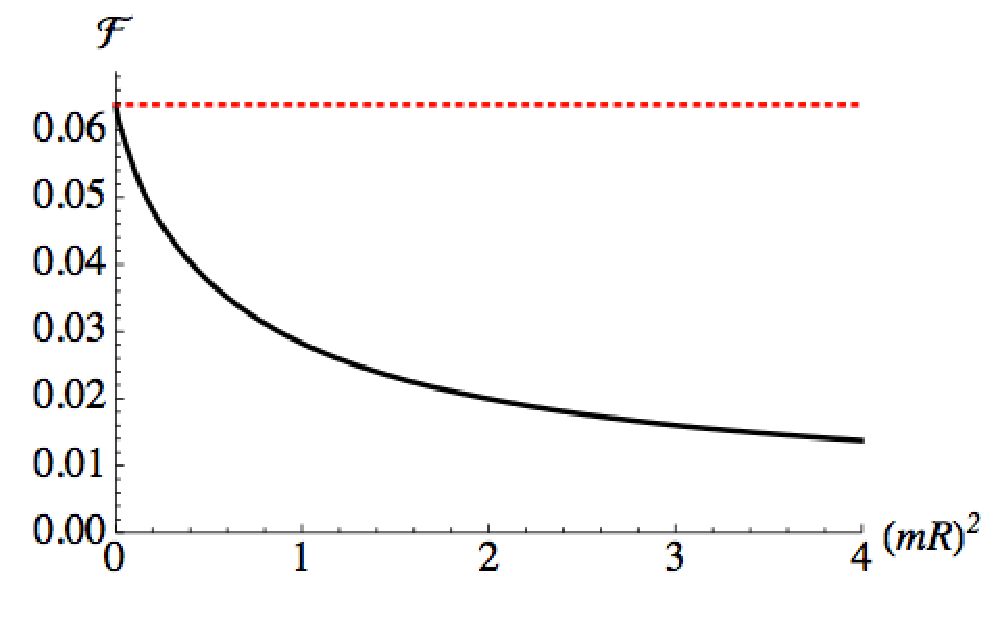
\includegraphics[width=8cm]{REEmassive.pdf}
\caption{The numerical plot of the $\CF$-function of a free massive scalar field (the black curve).
The dotted red line is the UV fixed point value $\CF_\text{UV}\approx 0.064$ of the $\CF$-function.
}
\label{fig:REEmassive}
\end{figure}



\subsubsection{Stationarity at UV fixed points}
Having dealt with the IR expansion of the $\CF$-function of the free massive scalar field, we look into the UV behavior around $m=0$.\footnote{See \textcite{Hertzberg:2012mn} for the case of an interacting scalar field theory.}
We see from the numerical plot in Fig.\,\ref{fig:REEmassive} that the derivative of $\CF$ is not stationary even at the UV fixed point when the free massive scalar field theory is considered as the relevant perturbation of a free massless scalar field theory by the mass term $m^2\phi^2/2$ \cite{Klebanov:2012va,Nishioka:2014kpa}.
This should be contrasted with Zamolodchikov's $c$-function that is guaranteed to be stationary at conformal fixed points.
The lack of stationarity is not peculiar to the $\CF$-function. 
Indeed, the entropic $c$-function Eq.\,\eqref{Entropic_C} of a massive free scalar field in two-dimensions is also known to be nonstationary at the UV fixed point \cite{Casini:2005zv}.

One may wonder if the nonstationarity is a generic feature for the entropic $c$- and $\CF$-functions, independent of the types of QFTs.
To inspect it a little more, let $\CO(x)$ be a relevant scalar operator of dimension $\Delta\, (\le d)$ in $d$-dimensional CFT and consider the relevant perturbation by the operator
\begin{align}
	I_E = I_\text{UV} + g_\CO\, \int \d^d x\,\sqrt{g}\,\CO(x) \ ,
\end{align}
which induces an RG flow from the UV fixed point theory described by the action $I_\text{UV}$ to an IR fixed point.
The perturbative expansion of entanglement entropy around the UV fixed point $(g_\CO =0)$ should take the form,
\begin{align}\label{CP_EE}
	S (g_\CO) = S_\text{UV} + s_1\, g_\CO + s_2\,g_\CO^2 + O(g_\CO^3) \ .
\end{align}
The leading order term is the integrated two-point function of the modular Hamiltonian $H_A$ and the relevant operator \cite{Rosenhaus:2014woa,Rosenhaus:2014zza},
\begin{align}\label{s1}
	s_1 = - 2\pi\,\int \d^d x\,\sqrt{g}\, \langle H_A\, \CO(x)\rangle \ . 
\end{align}
The modular Hamiltonian is nonlocal in general, but can be expressed as the integral of a local integrand proportional to the stress tensor for a planar or spherical entangling surface in CFT as given in Eq.\,\eqref{Modular_Hamiltonian}.
In this case, the first-order term is expected to vanish, $s_1=0$, for $\langle T_{\mu\nu}(x)\,\CO(y)\rangle = 0$ in CFT (see Eq.\,\eqref{TO_CFT}) \cite{Rosenhaus:2014woa}.
Thus this perturbative argument shows quite generally that entanglement entropy is \emph{stationary} at the UV fixed point.
We record for the reader's reference that the second-order term $s_2$ is nonvanishing, whose form is determined for a spherical entangling surface of radius $R$ on $\BR^d$ to be \cite{Faulkner:2014jva}
\begin{align}
	s_2 = - R^{2(d-\Delta)} \frac{\pi^{(d+1)/2}(d - \Delta)\Gamma\left( d/2+1 - \Delta\right)}{2\Gamma \left( d+ 3/2 - \Delta\right)} \ ,
\end{align}
for operators with $\Delta \ge d/2$.

The contradiction between the presented general argument and the numerical result for a free massive scalar field needs some explanation.
The origin of this puzzle may be traced back to our tacit assumption for the stress tensor being conformal invariant, i.e., $T^\mu_{~\mu} = 0$ in deriving the expansion Eq.\,\eqref{CP_EE} with the conformal perturbation theory.
For a free scalar field, however, we have a family of the stress tensors $T^{(\xi)}_{\mu\nu}$ parametrized by a coupling constant $\xi$ for the curvature coupling $\CR\, \phi^2$ that can be added to the action when lifting the theory from flat spacetime to a curved spacetime.
$T^{(\xi)}_{\mu\nu}$ is conformally invariant (traceless) only when $\xi = \xi_c \equiv (d-2)/\left(4 (d-1)\right)$ even on flat spacetime.
There is no a priori reason to prefer the conformal stress tensor $T^{(\xi_c)}_{\mu\nu}$ to the others in calculating entanglement entropy.
The possibility of adopting the nonconformal stress tensors was examined by \textcite{Lee:2014zaa,Casini:2014yca,Herzog:2016bhv}, resulting in the speculation that the correct value of the leading coefficient $s_1$ is given by Eq.\,\eqref{s1} with the stress tensor $T^{(\xi = 0)}_{\mu\nu}$ for the minimal coupling $\xi = 0$.

Furthermore, the stationarity of entanglement entropy is conjectured to break down when there exists an operator $\CO_{d-2}$ of dimension $\Delta = d-2$ that can couple to the scalar curvature $\CR\,\CO_{d-2}$ \cite{Herzog:2016bhv}.
It remains to be clarified under what condition the entropic $c$- and $\CF$-functions become the stronger version of a $\CC$-function.




\subsection{The entropic $\CC$-theorems in $d\ge 4$ dimensions}\label{ss:C_theorem_Higher}
We have seen that the entropic $c$- and $F$-theorems in $(1+1)$ and $(2+1)$ dimensions follow from the strong subadditivity of entanglement entropy and the Lorentz invariance of QFTs.
One may then expect the $a$-theorem in $(3+1)$ dimensions similarly follows from the same argument. 
There however are two obstacles in the generalization to the higher-dimensional cases: i) the strong subadditivity inequalities become trivial due to logarithmic divergences coming from singular surfaces of intersecting boosted spheres, and ii) there is a finite mismatch between the entanglement entropies of the wiggly spheres and the round spheres in taking the number $N$ of the boosted spheres to infinity.

To overcome these difficulties, \textcite{Casini:2017vbe,Lashkari:2017rcl} considered a difference of the entanglement entropies across a $(d-2)$-sphere of radius $R$ between a theory $\CT$ along an RG flow and the UV CFT at its UV fixed point in $d$ dimensions,
\begin{align}
	\Delta S_\CT (R) \equiv S_\CT(R) - S_\text{UV}(R) \ ,
\end{align}
and define a new entanglement measure,
\begin{align}\label{S_function}
	\CS_\CT (R) \equiv \left[ R\,\partial_R -(d-2)\right] \Delta S_\CT (R) \ .
\end{align}
The strong subadditivity Eq.\,\eqref{SSA_general} still holds for the difference $\Delta S_\CT (R)$ thanks to the Markov property of the CFT vacuum that saturates the strong subadditivity for entangling regions whose boundaries are located on a light cone \cite{Casini:2017roe}.
Furthermore, this subtraction plays a twofold role to solve the problems: i)
the UV divergences from the singular intersections are canceled out in the difference $\Delta S_\CT (R)$, and ii) the wiggly spheres can be replaced by the round spheres in the strong subadditivity as the finite mismatch of their entropies cancels out in $\Delta S_\CT (R)$ \cite{Casini:2018kzx}.\footnote{We thank Eduardo Test{\'e} for clarifying this point.}
Hence taking the large $N$ limit of Eq.\,\eqref{SSA_general} with $S$ replaced with $\Delta S_\CT$ results in the monotonicity of $\CS_\CT (R)$ in any dimension,
\begin{align}\label{S_function_Mon}
	\CS'_\CT (R) \le 0 \ .
\end{align}
This new measure reduces to the entropic $c$- and $\CF$-functions when $d=2$ and $3$, respectively, and the inequality \eqref{S_function_Mon} guarantees their monotonicities.

Now we move onto the four-dimensional case and see what we are able to draw from the inequality \eqref{S_function_Mon}.
Recalling Eqs.\,\eqref{EE_4d} and \eqref{c04d}, the entanglement entropy across a two-sphere of radius $R$ in CFT$_4$ is given by
\begin{align}\label{EE_4d_CFT}
	S(R)|_\text{CFT} = \alpha\,\frac{4\pi R^2}{\epsilon^2} - a\, \log \frac{R}{\epsilon} \ .
\end{align}
We are interested in the difference of the $a$-anomalies between the UV and IR fixed points of an RG flow and hence consider the IR CFT as a theory $\CT$ for the measure $\CS_\CT (R)$.
Evaluating the inequality \eqref{S_function_Mon} with the fixed point value Eq.\,\eqref{EE_4d_CFT} we find
\begin{align}
	\CS_\text{IR}'(R) = 2 (a_\text{IR} - a_\text{UV}) \frac{1}{R} \le 0 \ ,
\end{align}
which proves the weak version of the $a$-theorem Eq.\,\eqref{a_theorem_claim}  \cite{Casini:2017vbe}.\footnote{The dilation effective action was used by \textcite{Solodukhin:2013yha} to prove the $a$-theorem using the entanglement entropy of a spherical entangling surface.
}

In $d\ge 4$ dimensions \textcite{Giombi:2014xxa} conjectured the generalized $F$-theorem, stating the generalized $F$ coefficient defined by
\begin{align}
	\tilde F \equiv \sin \left( \frac{\pi\,d}{2}\right)\, \log\,Z[\BS^d] \ ,
\end{align}
decreases along an RG flow,
\begin{align}\label{Generalized_F}
	\tilde F_\text{UV} \ge \tilde F_\text{IR} \ .
\end{align}
We want to examine if the monotonicity Eq.\,\eqref{S_function_Mon} in $d\ge 4$ dimensions also proves the conjecture as in the lower-dimensional cases.

Noting the small $R$ limit that corresponds to the UV region of an RG flow, we found $\CS_\CT (0) = 0$ for any theory $\CT$.
Then the inequality Eq.\,\eqref{S_function_Mon} implies
\begin{align}\label{S_IR_Monotonic}
	\CS_\CT (R) \le 0 \ .
\end{align}
By choosing $\CT$ to be the IR theory, it leads to an inequality that contains the UV divergence of order $O(1/\epsilon^{d-4})$ as seen from the UV structures Eqs.\,\eqref{EE_Even} and \eqref{EE_Odd} in CFT.
Hence we are not able to derive a relation between finite values of the form, Eq.\,\eqref{Generalized_F}.

One can still hope to regularize the UV divergence in Eq.\,\eqref{S_IR_Monotonic} by the dimensional regularization and derive the finite relation \eqref{Generalized_F}.
Indeed the equality Eq.\,\eqref{EE_F} leads to
\begin{align}
	\tilde F|_\text{CFT} = \sin \left( \frac{\pi\,d}{2}\right)\, S_\text{CFT}(R) \ ,
\end{align}
and one can recast Eq.\,\eqref{S_IR_Monotonic} into the inequality for the fixed point values $\tilde F_\text{UV}$ and $\tilde F_\text{IR}$.
While the resulting inequality agrees with Eq.\,\eqref{Generalized_F} for $2< d < 4$, it becomes rather the opposite, $\tilde F_\text{IR} \ge \tilde F_\text{UV}$ for $4 < d < 6$, which is in apparent contradiction to the free field results \cite{Giombi:2014xxa}.
This conflict stems from the fact that the inequality Eq.\,\eqref{S_IR_Monotonic} holds only in the presence of the UV divergences.
It is challenging, at the time of writing this review, to derive an inequality for the dimensionally regularized entanglement entropies, which hopefully proves the generalized $F$-theorem in higher dimensions.


\subsection{Holographic RG flow}

In this section, we switch gears to consider a simple class of holographic RG flows that are dual to Lorentz invariant QFTs in $d$ dimensions and examine the entanglement entropy across a sphere under the flows \cite{Liu:2012eea,Klebanov:2012yf,Liu:2013una}.
A complementary test of the $F$-theorem in three dimensions is performed in the holographic systems.


\subsubsection{Domain wall and gapped RG flows}
The most general metric holographically describing an RG flow on a flat space $\BR^{1,d-1}$ is of Poincar{\' e} type:
\begin{align}\label{RGmetric}
\d s^2 = \frac{L^2}{z^2}\left[  \frac{\d z^2}{f(z)} - \d t^2 + \d{\vec x}^2_{d-1} \right] \ ,
\end{align}
where $\d {\vec x}^2_{d-1}$ is the metric of the $(d-1)$-dimensional flat space $\BR^{d-1}$.
We require the function $f(z)$ approaches to a constant (that we choose to $1$ here),
\begin{align}\label{fto1}
f(z) \xrightarrow[z\to 0]{}1 \ ,
\end{align}
so that the metric asymptotes to an AdS$_{d+1}$ space-time of radius $L$ near the boundary $z=0$.

We are interested in a physical situation where the metric is a solution to the Einstein equation, so hence not every function $f(z)$ satisfying Eq.\,\eqref{fto1} is of interest.
Moreover we should exclude unphysical solutions by introducing a physically sensible condition.

Suppose the metric \eqref{RGmetric} describing an RG flow is a solution in the Einstein gravity coupled to matter fields,
\begin{align}
I = \frac{1}{16\pi G_N} \int \d^{d+1} x \sqrt{-g} \left[ \CR + \CL_\text{matter} \right] \ ,
\end{align}
where $\CL_\text{matter}$ is the Lagrangian of the matter fields.
The metric Eq.\,\eqref{RGmetric} with an arbitrary function $f(z)$ can be a solution to the Einstein equation,\footnote{Our definition of the stress tensor in Lorentzian signature is $T_{\mu\nu} = (2/\sqrt{-g})\,\delta I/ \delta g^{\mu\nu}$.} $T_{\mu\nu}^\text{matter} = \CR_{\mu\nu} - \CR g_{\mu\nu}/2$, by tuning the bulk matter stress tensor $T_{\mu\nu}^\text{matter}$ or equivalently the matter Lagrangian $\CL_\text{matter}$ properly.
This construction, however, often leads to unreasonable solutions that we may want to rule out on a physical ground.
It is common practice to impose the \emph{null energy condition} for making a theory of gravity physically sensible, \cite{Hawking:1973uf}:
\begin{align}\label{NEC}
T_{\mu\nu}^\text{matter} \xi^\mu \xi^\nu \ge 0 \ .
\end{align}
This condition must be met for any future directed null vector $\xi^\mu$ ($\xi^2 = 0$).


Using the Einstein equation $T_{\mu\nu}^\text{matter} = \CR_{\mu\nu} - \CR\, g_{\mu\nu}/2$ and the null vector of the form
\begin{align}\label{NVector}
\xi^z = \sqrt{f(z)} \ , \qquad \xi^t = 1 \ , \qquad \xi^i = 0 \qquad (i\neq t, z) \ ,
\end{align}
one can derive from the null energy condition a constraint,
\begin{align}\label{fmonotonic}
f'(z) \ge 0 \ ,
\end{align}
which implies the monotonicity of $f(z)$.
This constraint Eq.\,\eqref{fmonotonic} restricts a class of solutions available to us, but
is not strong enough to fix the IR geometry in the large $z$ region.
Here we consider the following two possibilities in the $z\to \infty$ limit \cite{Liu:2012eea}:
\begin{enumerate}
\item
The IR geometry is a different fixed point from the UV. 
Namely, the metric \eqref{RGmetric} describes a domain wall between two AdS$_{d+1}$ solutions with radii $L$ and $L_\text{IR}$,
\begin{align}\label{Domain}
f(z) \xrightarrow[z\to \infty]{} \frac{L^2}{L^2_\text{IR}} > 1\ .
\end{align}
\item
The IR geometry is a confining or gapped phase when the metric described by Eq.\,\eqref{RGmetric} has the function with the IR boundary condition,
\begin{align}\label{Gapped}
f(z) \xrightarrow[z\to \infty]{}  b\, z^n \ , \qquad n>0 \ ,
\end{align}
where $b$ is a positive constant.
\end{enumerate}


Now we are concerned with a spherical entangling surface.\footnote{See \textcite{Myers:2012ed} for a similar calculation with an entangling surface of a strip type.}
It is convenient to choose the spatial metric to be in the polar coordinates:
\begin{align}
\d{\vec x}_{d-1}^2 = \d\rho^2 + \rho^2\, \d\Omega_{d-2}^2 \ .
\end{align}
Since the entangling surface is spherical, $\rho$ has to be a function of $z$ to respect the spherical symmetry.
Then the area functional is given by
\begin{align}\label{AreaFunctionalSphere}
\begin{aligned}
\CA &= L^{d-1}\,\text{Vol}(\BS^{d-2})\int_0^{z_\ast} \d z\, \CL\ ,\\
\CL &= \frac{\rho(z)^{d-2}}{z^{d-1}}\sqrt{\rho'(z)^2 + \frac{1}{f(z)}} \ ,
\end{aligned}
\end{align}
where $z_\ast$ is the maximum value of $z$ for the minimal surface.
To find a solution minimizing the area, we impose the boundary condition at the UV fixed point ($z=0$),
\begin{align}
\rho(z) = R + O(z^2) \ ,
\end{align}
while at the IR fixed point there are two types of boundary conditions depending on the topology of the minimal surface (see Fig.\,\ref{fig:Topology}).
\begin{figure}[htbp]
\centering
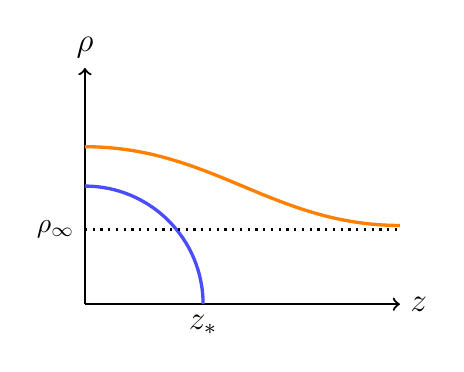
\begin{tikzpicture}[thick]
	\draw[->] (0,0) --++(4,0) node[right] {\large $z$};
	\draw[->] (0,0) --++(0,3) node[above] {\large $\rho$};
	\draw[very thick, blue!70] (1.5,0) node[below,black] {\large $z_\ast$} arc (0:90:1.5) ;
	\draw[very thick, orange] (0,2) to [out=0, in=180] (4,1);
	\draw[dotted] (0,0.95) node[left] {$\rho_\infty$} --++ (4,0);
\end{tikzpicture}

\caption{Two types of a minimal surface. The dashed blue and solid orange curves are disk and cylinder type surfaces, respectively.}
\label{fig:Topology}
\end{figure}
\begin{itemize}
\item
Disk type ($z_\ast < \infty$): 
the minimal surface terminates at $z=z_\ast$ where $\rho$ has the expansion of the form
\begin{align}
\rho(z) =  (z_\ast - z)^{1/2}\left[\rho_\ast + O (z_\ast - z) \right]\ .
\end{align}
\item
Cylinder type ($z_\ast = \infty$):
the minimal surface extends to the infinity as 
\begin{align}
\rho(z) = \rho_\infty + O(1/z) \ .
\end{align}
\end{itemize}
When $f(z)=1$, i.e., the AdS$_{d+1}$ spacetime, the minimal surface is of a disk type as we saw in Eq.\,\eqref{Sp_sol}:
\begin{align}\label{AdSDiskSol}
\rho_0(z) = \sqrt{R^2 - z^2} \ .
\end{align}
Hence we expect to have a disk type solution when the radius $R$ of the entangling surface is small in an asymptotically AdS spacetime.
On the other hand, a cylinder type solution can exist in a gapped geometry with the IR behavior Eq.\,\eqref{Gapped} only when $n>2$ [see Appendix C in \cite{Liu:2012eea} for details].


\subsubsection{Topology change in a gapped phase} 
The minimal surface in the asymptotically AdS spacetime Eq.\,\eqref{RGmetric} is approximated by the solution Eq.\,\eqref{AdSDiskSol} for small $R$.
If the bulk geometry allows the cylinder type minimal surface for large $R$, there must be a topology change at some critical value $R=R_c$.
This is actually a typical phenomenon for a gapped phase Eq.\,\eqref{Gapped} as one can verify as follows.

We can probe the IR region even for small $z$ by letting the parameter $b$ be very large, $b\gg 1$.
The large $b$ expansion of the equation of motion for the area functional Eq.\,\eqref{AreaFunctionalSphere} amounts to, in the leading order, either 
\begin{align}
	\rho'(z)=0 \ , 
\end{align}
or 
\begin{align}
	\rho'(z) = c\, z^{(d-1)/(d-2)} \ ,
\end{align}
for a constant $c$.
The solution to the second equation diverges for large $z$ and is not acceptable as a minimal surface
while the solution to the first implies a cylinder type minimal surface.
The topology change of the minimal surface is observed numerically in many examples \cite{Liu:2012eea,Klebanov:2012yf,Liu:2013una}.

The area of the cylinder type minimal surface may be evaluated in the system with a large gap ($b\gg 1$) by dividing the calculation into the UV part $z\leq z_b \equiv b^{-1/n}$ and the IR part $z> z_b$.
In the UV region, the solution is close to the disk solution Eq.\,\eqref{AdSDiskSol} in the AdS space while it approaches to a constant in the IR region.
Taking into account the continuity at $z=z_b$, it is reasonable to approximate the solution by the piecewise function,
\begin{align}
	\rho(z) = \begin{cases}
			\rho_0(z) & \quad (z\leq z_b) \ ,\\
			\rho_0(z_b) & \quad (z> z_b) \ .
			\end{cases}
\end{align}
Now the area consists of two parts, $\CA = \CA_{z\leq z_b} + \CA_{z\geq z_b}$, where the UV part is approximated in the large $b$ limit by
\begin{align}
\begin{aligned}
	\CA_{z\leq z_b} = \int_{\epsilon}^{z_b}\d z\,&\frac{\rho_0(z)^{d-2}(\rho_0'(z)^2 + 1)^{1/2}}{z^{d-1}} \\
		&\quad \cdot \left[ 1 - \frac{b\,z^n}{2(\rho_0'(z)^2 +1)}\right] \ ,
\end{aligned}
\end{align}
while	 the IR part becomes
\begin{align}
	\CA_{z\geq z_b} = \int_{z_b}^\infty \d z\, \frac{\rho_0(z_b)^{d-2}}{b^{1/2}\,z^{d-1 + n/2}} \ .
\end{align}
Using the dimensional regularization assuming $n$ is large enough, we have the expansion for $z_b\ll 1$,
\begin{align}\label{EE_Sphere_Gap}
	\CA &= \frac{1}{2d + n -4} \left[2 \left(\frac{R}{z_b}\right)^{d-2}  - (d-2) \left(\frac{R}{z_b}\right)^{d-4} + \cdots \right] \ .
\end{align}
The entanglement entropy across a sphere of radius $R$ is $L^{d-1}\text{Vol}(\BS^{d-2})/(4G_N)$ times larger that this area.
Compared with Eq.\,\eqref{EE_Scalar_HK} for a free massive scalar field, the parameter $z_b$ allows for interpretation as a gap scale $m$ as expected.


Similar topology change can be observed for a strip entangling region in a gapped system where the entangling surface is two parallel planes.
There are two types of extremal surfaces, one with a connected surface, and the other with two disconnected surfaces terminate on the IR boundary of the gapped geometry.
The topology change between these two types of surfaces is interpreted as a confinement/deconfinement phase transition in a confining gauge theory \cite{Nishioka:2006gr,Klebanov:2007ws,Pakman:2008ui}.


\subsubsection{Testing the $F$-theorem in holography}
As seen in Sec. \ref{ss:Ftheorem}, the proof of the $F$-theorem was based on the Lorentz invariance and the strong subadditivity of entanglement entropy that replaces the role of unitarity in QFT. 
The same argument for the proof remains to work in a holographic system as well just by resorting to the strong subadditivity of the Ryu-Takayanagi formula (for the static case in Sec. \ref{ss:HEE_Ineq}).
Nevertheless, it is worthwhile examining the validity of the $F$-theorem from  the holographic point of view to draw implications for the interplay between unitarity in QFT and its counterpart in the dual gravity.

First let us consider a holographic gapped system with a large gap
that we dealt with in the previous section.
The renormalized entanglement entropy, Eq.\,\eqref{REE}, across a sphere of large radius is calculated from Eq.\,\eqref{EE_Sphere_Gap} with $d=3$ as,
\begin{align}\label{HREE_Gap}
	\CF(R) = \frac{\pi\,L^2}{(n+2)\,G_N}\frac{z_b}{R} + O\left( (z_b/R)^{3}\right) \ .
\end{align}
This result should be compared with the typical behavior of the $\CF$-function in the large gap limit given in Eq.\,\eqref{LargeMassExpansionScalar} for a free massive scalar.
Note that the value of $\CF$ (the sphere free energy) at the UV fixed point of the holographic RG flow is $F_\text{UV} = \pi L^2/(2G_N)$ [see Eq.\,\eqref{CFT_F_value}], which is always greater than Eq.\,\eqref{HREE_Gap} in the large gap system with $z_b \ll R$.
We thus find this type of holographic RG flow is consistent with the $F$-theorem.


The next example to consider is a domain wall RG flow interpolating two closely separated fixed points without a gap \cite{Liu:2012eea}.
Such a solution can be realized by choosing the function $f(z)$ in the general metric Eq.\,\eqref{RGmetric} to be of the form
\begin{align}
\begin{aligned}
f(z) &= 1 + \eta\, g(z) \ , \qquad \eta = \frac{L^2}{L_\text{IR}^2} - 1 \ll 1 \ , 
\end{aligned}
\end{align}
and imposing the boundary conditions at the UV and IR regions,
\begin{align}
	 g(z) &\xrightarrow[z\to 0]{}0 \ ,\qquad g(z) \xrightarrow[z\to \infty]{}1 \ .
\end{align}
The null energy condition Eq.\,\eqref{fmonotonic} indicates $g(z)$ to be a monotonically increasing function,
\begin{align}\label{Mon_g}
	g'(z)\ge 0 \ .
\end{align}
In this setup, we are allowed to expand the solution of the equation of motion of the area functional Eq.\,\eqref{AreaFunctionalSphere} around the UV solution Eq.\,\eqref{AdSDiskSol},
\begin{align}
\rho(z) = \rho_0(z) + \eta\, \rho_1(z) + O(\eta^2) \ ,
\end{align}
and it follows the expansion of the area functional,
\begin{align}
\CA = A_0 + \eta \,A_1 + O(\eta^2) \ .
\end{align}

We now focus on the $d=3$ case to inspect the behavior of the $\CF$-function.
Varying Eq.\,\eqref{AreaFunctionalSphere} around the UV solution, we obtain the subleading term of the form\footnote{There are contributions from the boundaries at $z=z_\ast$ and $0$, which turns out to be negligible for $d\le 4$ \cite{Liu:2012eea}.}
\begin{align}
\begin{aligned}
A_1 &= 2\pi L^{2}\int_0^{R} \d z\, g(z)\, \frac{\delta \CL}{\delta f}\bigg|_{f=1,\,\rho=\rho_0} \ , \\
	&= - \frac{\pi L^2}{R} \int_0^R \d z\, \frac{R^2 - z^2}{z^2}\,g(z) \ .
\end{aligned}
\end{align}
This integral is UV divergent due to the contribution near the UV boundary, $z=0$,
but we can regularize it with the $\CF$-function and find the leading correction,
\begin{align}\label{DWF}
\D\CF (R) = -\eta\, \frac{\pi L^2}{2G_N} \int_0^1 \d z \, g(zR) \ .
\end{align}
which is always nonpositive due to Eq.\,\eqref{Mon_g}.
We thus find the $\CF$-function of the domain wall solution decreases as $R$ increases.
Furthermore, the leading correction matches the difference between the UV and IR free energies,
\begin{align}
\begin{aligned}
\D \CF (R\to\infty) &= -\eta\, \frac{\pi L^2}{2G_N}\ , \\
	& = F_\text{IR} - F_\text{UV} + O(\eta^2)\ .
\end{aligned}
\end{align}
Hence the domain wall RG flow realizes the strong version of the $F$-theorem.\footnote{The entanglement entropy of a holographic RG flow describing a relevantly perturbed CFT is shown to have the expansion of the form \eqref{CP_EE} with $s_1=0$ and supports the strongest version of the $F$-theorem at least around the UV fixed point when the dimension of the relevant operator is close to $3$ \cite{Taylor:2016aoi,Taylor:2016kic}.}

We note that the monotonicity of the $\CF$-function is a direct consequence of the null energy condition Eq.\,\eqref{fmonotonic} in this holographic RG flow while it follows  in the field theoretic derivation in section \ref{ss:Ftheorem} from the strong subadditivity that is substituted by the minimality condition for the Ryu-Takayanagi surface.
The derivation for Eq.\,\eqref{DWF} indicates that the minimality condition is not enough to prove the monotonicity of the $\CF$-function in holography.
To our best knowledge, no holographic proofs of the strong version of the $F$-theorem are known, hence 
it is desirable to elucidate it with the null energy condition along the line of \textcite{Freedman:1999gp,Girardello:1998pd} beyond the perturbative level.


\subsection{Supersymmetric R{\'e}nyi entropies}\label{ss:SRE}
We conclude this section with a comment on some exact results for entanglement and R{\'e}nyi entropies in interacting field theories with supersymmetries.

Calculating the exact value of entanglement entropy in QFTs is generally an intractable task unless theories are free and the entangling surface preserves a rotational symmetry around it.
The difficulty is most manifest in the replica method where the conical singularity on the entangling surface prevents us from carrying out the perturbative calculation in a conventional manner.
On the other hand, there are powerful computational techniques, called \emph{supersymmetric localizations}, in supersymmetric field theories that allow the exact calculation of the partition function and a certain class of correlation functions by reducing the infinite-dimensional path integral to a finite-dimensional one \cite{Willett:2016adv,Dumitrescu:2016ltq,Pufu:2016zxm}.
To apply supersymmetric localization, a supersymmetric field theory must be placed on manifolds preserving enough number of supersymmetries.

A simple example is a round sphere and the resulting supersymmetric partition function $Z^\text{susy}[\BS^d]$ turns out to be the partition function $Z[\BS^d]$ of the supersymmetric field theory at the IR fixed point.
Given the relation \eqref{EE_F} between the entanglement entropy across a round sphere and the sphere partition function $Z[\BS^d]$ for CFTs, it is possible to calculate the exact value of entanglement entropy for a class of supersymmetric field theories \cite{Jafferis:2011zi,Pufu:2016zxm}.

Given the success of the entanglement entropy, one may wonder if the same story applies to the R{\'e}nyi entropy, Eq.\,\eqref{Renyi_QFT}, for supersymmetric field theories as well.
Such an attempt would fail as supersymmetries are completely broken on the $n$-fold cover of the $d$-sphere $\BS^d_n$ [defined by Eq.\,\eqref{CFT_Sphere}], thus the supersymmetric localization cannot be applied.

In order to leverage the supersymmetric localization technique, we would rather tailor the definition of the R{\'e}nyi entropy so as to be compatible with supersymmetries.
Namely, we define the \emph{supersymmetric R{\'e}nyi entropy} $S_n^\text{susy}$ for supersymmetric conformal field theories by \cite{Nishioka:2013haa},
\begin{align}\label{SRE_def}
	S_n^\text{susy} \equiv \frac{1}{1-n} \log \bigg| \frac{Z^\text{susy}[\BS^d_n]}{(Z^\text{susy}[\BS^d])^n} \bigg| \ ,
\end{align}
where $Z^\text{susy}[\BS^d]$ is the supersymmetric partition function on $\BS^d_n$ with background fields turned on to preserve a part of supersymmetries.\footnote{The effect of the background fields vanishes for CFT on a round sphere, hence $Z^\text{susy}[\BS^d] = Z[\BS^d]$.}
This definition takes the same form as the R{\'e}nyi entropy Eq.\,\eqref{Renyi_QFT} across a spherical entangling surface $\BS^{d-2}$ in CFT on $\BR^d$ [see Eq.\,\eqref{F_nZ}], except for the partition function being replaced with the supersymmetric one.\footnote{
The absolute value inside the logarithm ensures that the supersymmetric R{\'e}nyi entropy is universal at least in three dimensions \cite{Closset:2012vg}.}

The explicit formula for $Z^\text{susy}[\BS^d]$ is given by an integration over finite-dimensional matrix variables that depends on the spacetime dimensions, the rank of the gauge group, and the matter contents of supersymmetric field theories, but we are not concerned with the explicit form here.
Instead of giving examples, we recap the universal aspects of the supersymmetric R{\'e}nyi entropy for $\CN= 2$ supersymmetric field theories with the global $\U(1)_R$ symmetry in three dimensions \cite{Nishioka:2013haa}:
\begin{itemize}
\item The expansion around $n=1$ takes the form
\begin{align}
	S_n^\text{susy} = S_1 + \frac{\pi^2}{16}\,\tau_{RR}\,(n-1) + O\left((n-1)^2 \right) \ ,
\end{align}
where $\tau_{RR}$ appears as the coefficients $C_J = \tau_{RR}/(4\pi^2)$ and $C_T = 3 \tau_{RR}/(2\pi^2)$ in the correlators of the $\U(1)_R$-symmetry current $j_\mu^{(R)}$ and the stress tensor given by Eqs.\,\eqref{jjCor} and \eqref{TTCor}.
Compared with the expansion Eq.\,\eqref{REexpand} of the R{\'e}nyi entropy with the first derivative Eq.\,\eqref{LeadingRE} in $d=3$ dimensions,  
\begin{align}
	S_n = S_1 + \frac{\pi^2}{8}\, \tau_{RR}\,(n-1) + O\left((n-1)^2 \right) \ ,
\end{align}
we find a factor $2$ discrepancy at the leading order coefficient.
This is due to the effect of the background gauge field for the $\U(1)_R$ symmetry that is turned on to maintain supersymmetries on $\BS^d_n$. 
Hence the supersymmetric R{\'e}nyi entropy is \emph{different} from the R{\'e}nyi entropy when $n\neq 1$ in general.
\item For theories with gauge groups of rank $N$, the $n$ dependence simplifies in the large-$N$ limit,
\begin{align} 
	S_n^\text{susy} = \frac{3n+1}{4n}\, S_1 \ ,
\end{align}
A curious fact is that the ratio $H_n\equiv S_n^\text{susy}/S_1$ satisfies the inequalities Eqs.\,\eqref{RenyiIneq1}-\eqref{RenyiIneq4} of the R{\'e}nyi entropies.
\item For a certain class of superconformal field theories allowing for the holographic dual description, the gravity dual of the supersymmetric R{\'e}nyi entropy is described by the charged topological AdS$_4$ black hole that is a half-BPS solution in the $\CN= 2$ $\U(1)$ gauged four-dimensional supergravity \cite{Nishioka:2014mwa,Huang:2014gca}.
\item The description by codimension-two defects living on the entangling surface is manifest \cite{Nishioka:2016guu}.
\end{itemize}


The supersymmetric R{\'e}nyi entropies and their gravity duals have been explored with applications in the other dimensions \cite{Mori:2015bro,Giveon:2015cgs,Huang:2014pda,Zhou:2015cpa,Hama:2014iea,Alday:2014fsa,Nian:2015xky,Zhou:2015kaj,Yankielowicz:2017xkf}.
We believe they shed new light on understanding the nature of quantum entanglement in QFT and the fundamental connection of quantum states to the holographic spacetime.


\endinput